% Include Packages
\documentclass[a4paper]{article}
\usepackage{fancyhdr}
\usepackage{extramarks}
\usepackage{graphicx, xcolor, wrapfig}
\usepackage[a4paper, tmargin=1cm, bmargin=2cm]{geometry}
\usepackage[utf8]{inputenc}
\usepackage[justification=centering]{caption}
\usepackage[intlimits]{amsmath}
\usepackage{amssymb}
\usepackage[american]{circuitikz}
\usepackage{pdflscape}
\usepackage{listings}
\usepackage{hyperref}
\usepackage{caption}
\usepackage{subcaption}
\usepackage{float}
\usepackage{color}
\usepackage{booktabs}
\usepackage{multirow}

\usepackage[utf8]{inputenc}
\usepackage[english]{babel}
 
\usepackage{biblatex}
\addbibresource{refrence.bib}

%% Hyperlinks Coloring 
\hypersetup{
    colorlinks=true,
    linkcolor=blue,
    filecolor=magenta,      
    urlcolor=cyan,
}

%% Table Columns with Predefined Spacing
\usepackage{array}
\newcolumntype{L}[1]{>{\raggedright\let\newline\\\arraybackslash\hspace{0pt}}m{#1}}
\newcolumntype{C}[1]{>{\centering\let\newline\\\arraybackslash\hspace{0pt}}m{#1}}
\newcolumntype{R}[1]{>{\raggedleft\let\newline\\\arraybackslash\hspace{0pt}}m{#1}}

\renewcommand{\arraystretch}{1.25}


%% Setting Page Margins. required for fancyhdr to work properly
\topmargin=-0.45in
\evensidemargin=0in
\oddsidemargin=0in
\textwidth=6.5in
\textheight=9.0in
\headsep=0.25in


%% Fancy Page definitions
\pagestyle{fancy}
\fancyhf{}
\fancyhead[L]{\name}
%\fancyhead[C]{Top Center}
%\fancyhead[R]{\courseCode\ :\ \hwTitle}
\renewcommand{\headrulewidth}{0.4pt}
\fancyfoot[L]{\today}
%\fancyfoot[C]{\thepage}
\fancyfoot[R]{Page\ \thepage}
\renewcommand{\footrulewidth}{0.4pt}

\fancypagestyle{firststyle}
{
    \fancyfoot[L]{\today}
    %\fancyfoot[C]{\thepage}
    \fancyfoot[R]{Page\ \thepage}
    \renewcommand{\footrulewidth}{0.4pt}
    \renewcommand{\headrulewidth}{0mm}%
}

%%%%%%%%%%%%%%%%%%%%%%%%%%%%%%%%%%%%%%%%%%%%%%%%%%%%%%%%%%%%%%%%%%%%%%%%%%%%%%%%
%%                           Change Things Here                               %%
%%%%%%%%%%%%%%%%%%%%%%%%%%%%%%%%%%%%%%%%%%%%%%%%%%%%%%%%%%%%%%%%%%%%%%%%%%%%%%%%

%% Common things
\newcommand{\courseName}{VLSI Design Lab -EE705}
\newcommand{\hwTitle}{Progress Report}
\newcommand{\name}{Video Capture followed by Compression on FPGA}
\newcommand{\rollNo}{183076005,173079027,173079006}
%\newcommand{\courseCode}{EE705}
\newcommand{\instiName}{IIT Bombay}


%% Title 
\title{
    \thispagestyle{firststyle}
%\noindent\makebox[\linewidth]{\rule{\paperwidth}{0.4pt}}\\
\courseName \\
\textbf{Video Capture followed by Compression on FPGA}\\
\textbf{\hwTitle}}
\author{Simranjeet Singh\ \ \ Imtiyaz Ansari\ \ \ Akhil Gakhar\ \ \ Abhishek Kumar\\
(183076005)\ \ \ \ \ \ \ \  (174070026)\ \ \ \ \ \ \ \ (173079027)\ \ \ \ \ \ \ \  (173079006)}
\date{\today}

\begin{document}

\maketitle

\section{Introduction}
Video compression play a major roll in the new era of internet and high speed transfer. Our project is to interface the camera on FPGA followed by Video compression for fast and accurate compression. Our ultimate goal of video compression is the bit reduction of video for storage and transmission. We have researched about the various compression algorithm used currently and decided to implement the MPEG-4 (Moving Picture Expert Group)
Compression algorithm. We have tested the algorithm in python before implementing to FPGA(described in later section). In parallel we are interfacing the camera with FPGA.

\section{Algorithm}
Compression is the technique to reduce the number of bits used in frame. There are some information in the videos that we can not see so that we can throw such irrelevant data.
We can compress a video in two ways:
\begin{itemize}
    \item Lossy - A reasonable quality of video can reconstructed
    \item Lossless - Original video can be constructed 
\end{itemize}

We decided to use the MPEG-4 compression algorithm based on the complexity and compression parameters. MPEG-4 is good for video streaming and television broadcasting and capable of $1/50$ compression factor \cite{comp}. 
\subsection{Color System}
    This section describe the color system in the each frame of the image. Each frame of the video consists of 640x480 pixels. each pixel of the image is combination of different color to produce the different color. There are different ways of producing these color combinations:
    \begin{itemize}
        \item RGB: RGB is mos popular because the human eyes are easy to build up on these colors. Read green and blue color are available on each pixel. Data format of these color also vary. Normally 8-bit values to store each color. 
        \item HSV or HSL: This is the combination of color into hue, saturation and luminance. This is more natural way to describe the colors
        \item Y$C_rC_b$: This color space is used in the image and video compression because its reflects the fact that eyes are less sensitive to fine color detail of the \textbf{brightness}. In this color space one luma(y) component and two chroma($C_b$ and $C_r$) components are used to represent the image.
        \item Gray scale: In this value of each pixel is represented in the single sample representing the amount of light. This is kind of Black and white or monochrome images.
    \end{itemize}
In color Image or video compression Y$C_bC_r$ is used. We can convert the color from one color space to another using various formulas.

\subsection{Block Diagram}
This the simplest way of compress the Frame of video. We have tested our algorithm on gray scale image \cite{online}. 
\begin{figure}[H]
    \centering
    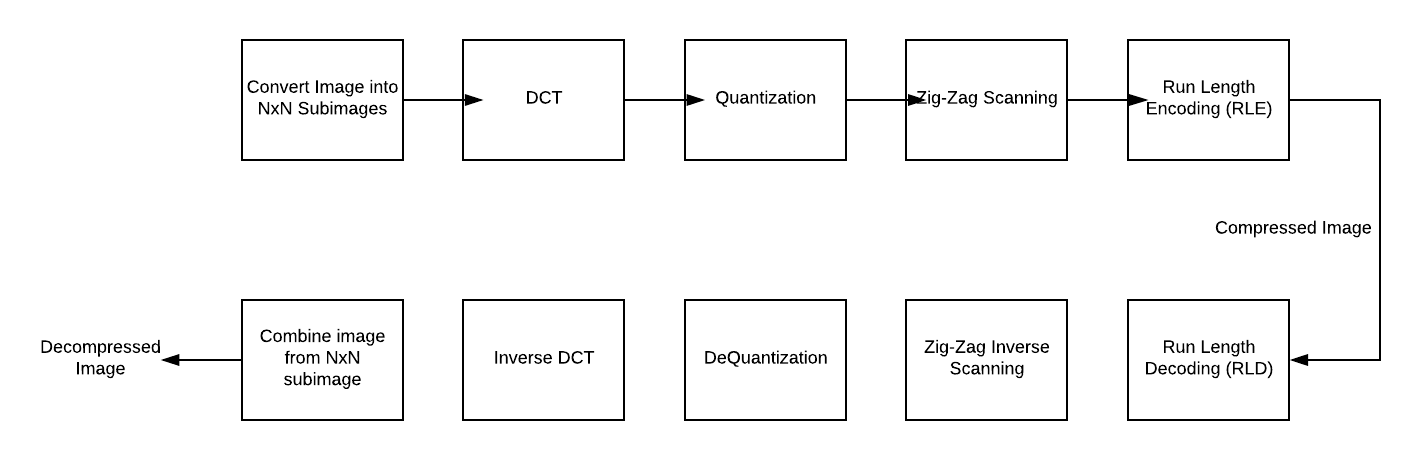
\includegraphics[width = \linewidth]{Blank_Diagram.png}
    \caption{Block Diagram of frame compression}
    \label{fig:my_label}
\end{figure}
\subsubsection{Covert Image into NxN sub image}
We convert the image into sub image to make the process faster. We have divided the image into 8x8 subimage and the further operation is applied on the 8x8 sub image. As our image resolution is 640x480 = 307200 pixel and now in sub image we have 8x8 = 64 pixel. Total sub images we got is $307200/64 = 4800 $. The DCT (Discrete cosine transform) is performed on each subimage
\subsubsection{DCT}
DCT- Discrete Cosine transform is conversion of pixel values into spatial frequency transformation in vertical and horizontal orientation. This transformation is performed on 8x8 subimage means 64 pixels. It will return the 64 frequency coefficients which means no data loss after DCT.\\
DCT is better than Fourier transform because the transformation is not periodic and neighboring pixel vaules are two different while Fourier transform assume the periodicity at the end of each block.\\
We have used the Opencv Function to convert the sub image into DCT. After DCT conversion each pixel value we got into $-128$ to $127$.\\
The following picture shows the transformation on DCT.
\begin{figure}[H]
    \centering
    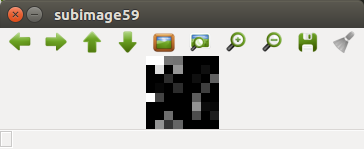
\includegraphics[width = \linewidth]{single_dct.png}
    \caption{DCT of Subimage}
    \label{fig:my_label}
\end{figure}

\begin{figure}[H]
    \centering
    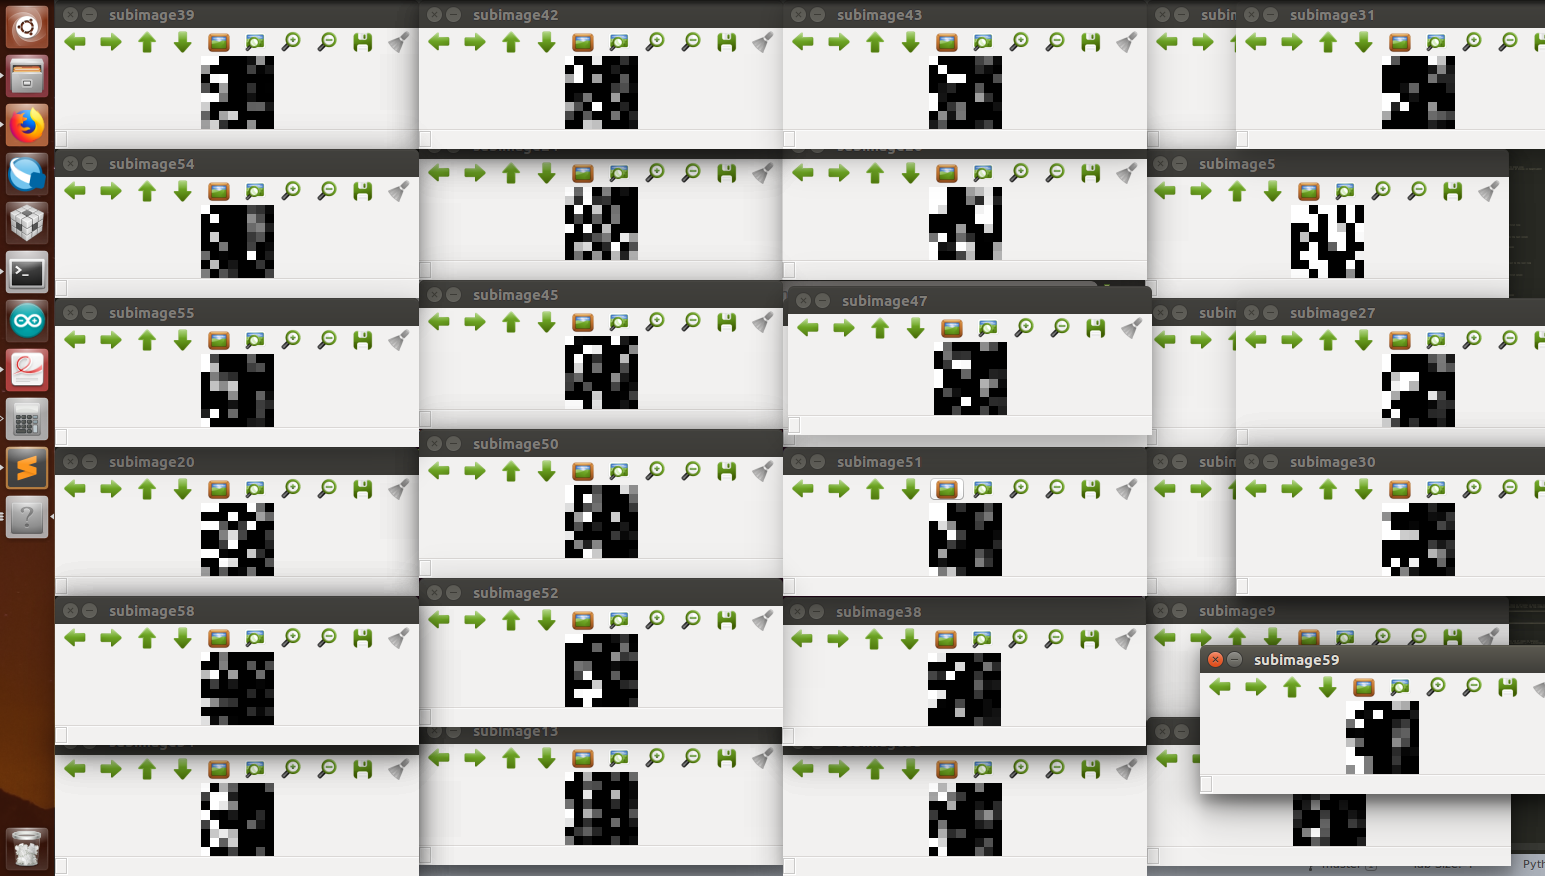
\includegraphics[width = \linewidth]{full_dct.png}
    \caption{DCT of Subimages}
    \label{fig:my_label}
\end{figure}
\subsubsection{Quantization}
This is the process to reduce the number of bits by divided the particular number. Suppose our values are varying between 0-255 means we have to use 8 bits to represents the range of value. if we divide the complete set of values by a factor(20) the range will be changed to 0 to 13 and we can represent this value into 4 bit. \\

In our case we have used the 8x8 matrix to divide the each pixel of the subimage by a factor. Each pixel of image subimage[0][0] to subimage[7][7] is divided by different set of value.\\
The same value should be used during the dequatization to retrieve the original value
\newpage

\subsubsection{Zig-Zag scanning}
Zig-Zag scanning is used to collect the number of values in the same order. Actually its a conversion of $2-D$ array of image into $1-D$ array so that Run length encoding can be perform. an example of this scanning is shown below:

\begin{figure}[H]
    \centering
    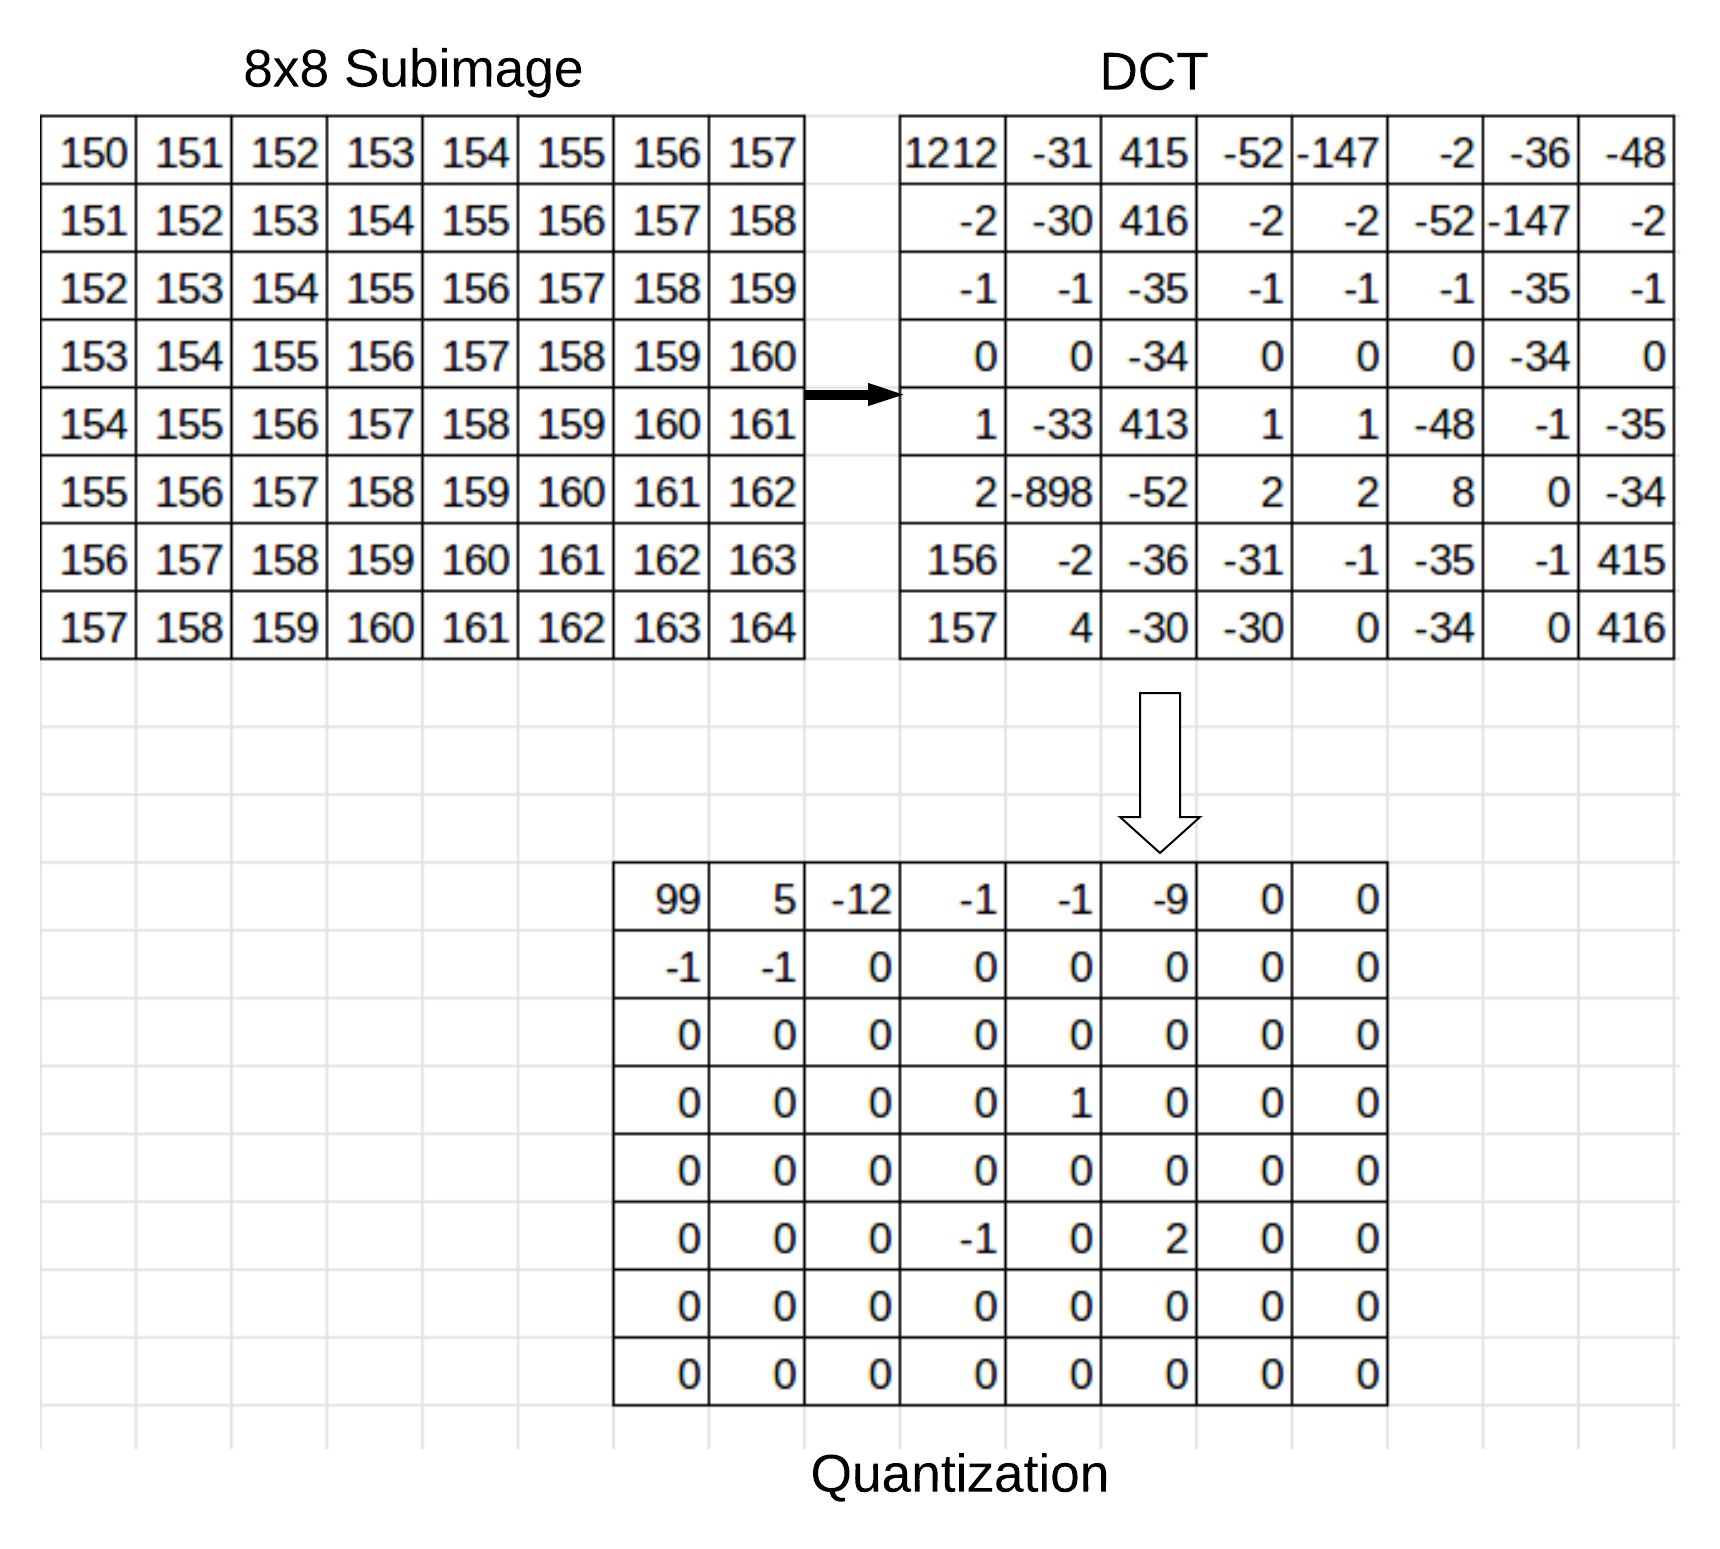
\includegraphics[width = \linewidth]{table.png}
    \caption{Conversion}
    \label{fig:my_label}
\end{figure}
Note: The above image data is dummy data for example.\\
As you can see the data after quantization in the table. There are number of zeros in the image matrix. we will scan this image in zig-zag manner so that number on zeros come together. this will help us to perform the run length encoding.


\begin{figure}[H]
    \centering
    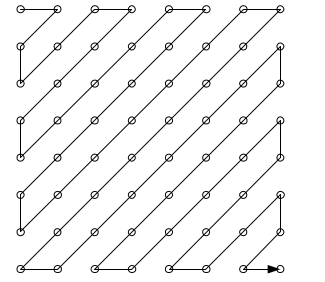
\includegraphics[scale=0.5]{zig-zag.png}
    \caption{Zig-Zag scanning of Image \cite{book}}
    \label{fig:my_label}
\end{figure}

Zig-Zag scanning return the $1-D$ array. [[data]] to [data]. Using this array i can perform the run length encoding. This scanning is perform on 8x8 subimage. Combined image after the zigzag scanned is shown below:

\begin{figure}[H]
    \centering
    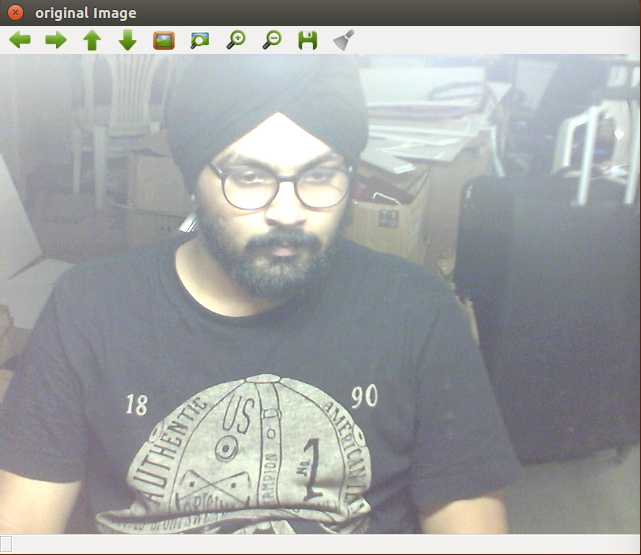
\includegraphics[scale=0.5]{original.png}
    \caption{Original Image}
    \label{fig:my_label}
\end{figure}

\begin{figure}[H]
    \centering
    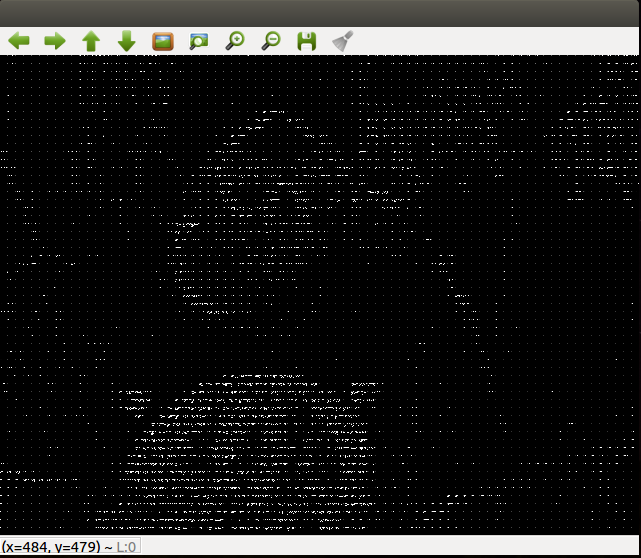
\includegraphics[scale=0.5]{encoded.png}
    \caption{Scanned image}
    \label{fig:my_label}
\end{figure}
You can see the original image is in the format of RGB. This image shown is without run length encoding and padded on the black image. You can observe the shape of body in the pixel.

\subsubsection{Run Length encoding(RLE)}
RLD is Lossless encoding used in the compression. As previously discussed we have changed the image into array. This image is stored in zig-zag manner. We can perform the encoding and reduce the number of bits.\\
\begin{itemize}
    \item Example: consider a screen containing plain black text on a solid white background. There will be many long runs of white pixels in the blank space, and many short runs of black pixels within the text. A hypothetical scan line, with B representing a black pixel and W representing white, might read as follows:

    WWWWWWWWWWWWBWWWWWWWWWWWWBBBWWWWWWWWWW\\
    WWWWWWWWWWWWWWBWWWWWWWWWWWWWW 

With a run-length encoding (RLE) data compression algorithm applied to the above hypothetical scan line, it can be rendered as follows:

    12W1B12W3B24W1B14W 
This would be interpreted as a run of twelve Ws, a B, a run of twelve Ws, a run of three Bs, etc. In data where runs are less frequent, this can significantly improve the compression rate
[Wikipedia of run length encoding]

We have implemented this run length encoding on the 640x480 image and converted it in small size (Exact compression size is to be measured).

\end{itemize}

\subsubsection{Decompression}

Decompression is done by reversing the each step mentioned in the block diagram and able to extract the original image. As we have done the compression n gray scale the final image will be in black and white format. Check the original image constructed from the final compressed video \cite{basic}.

\begin{figure}[H]
    \centering
    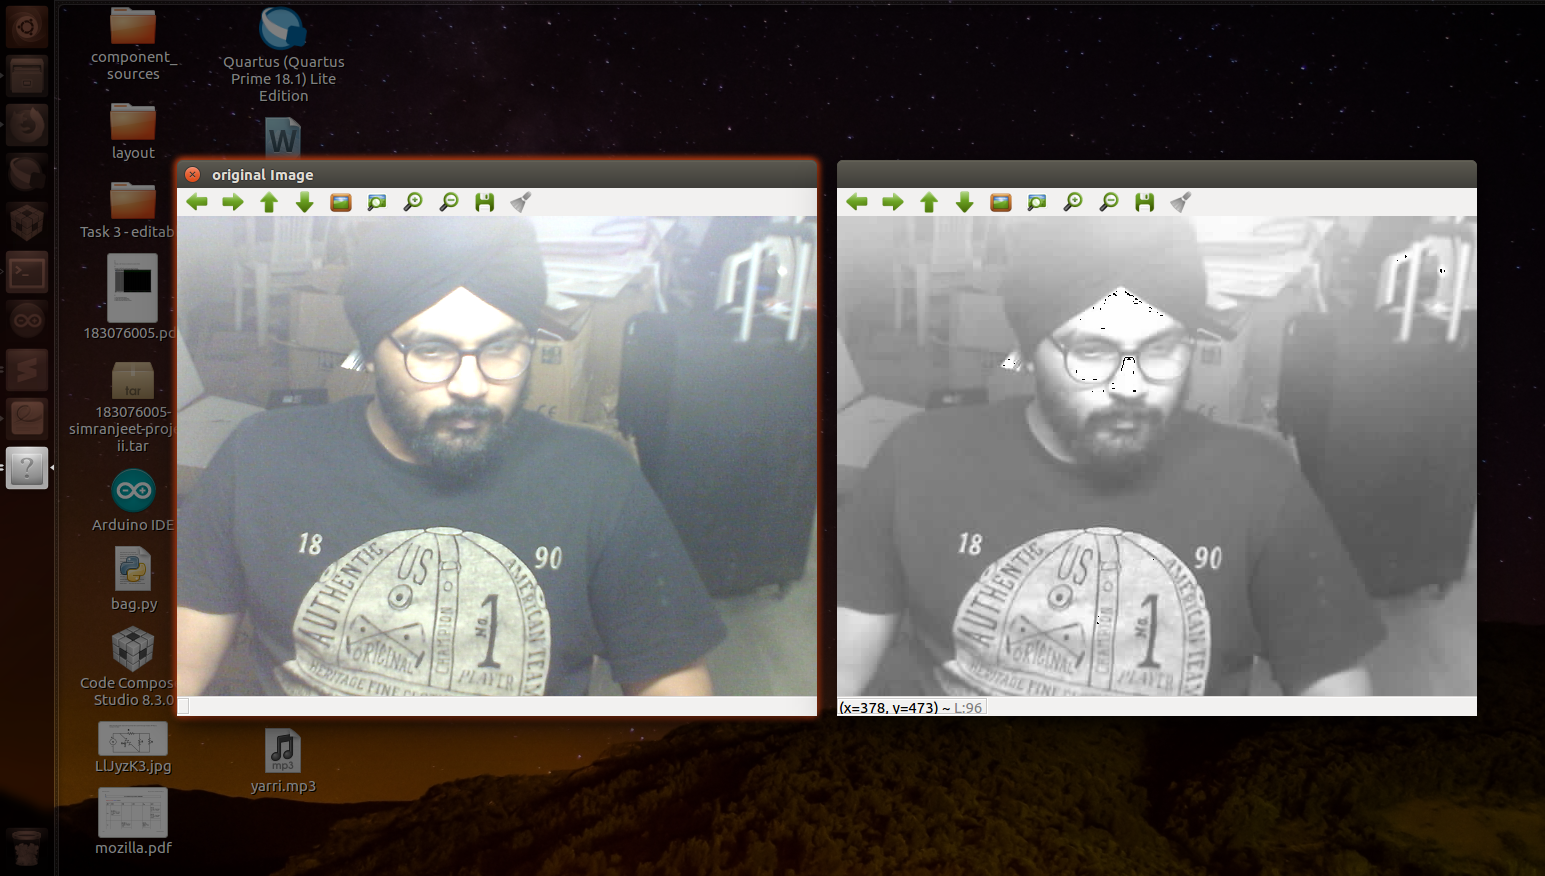
\includegraphics[scale=0.3]{image.png}
    \caption{Decompression}
    \label{fig:my_label}
\end{figure}
%%%%%%%%%%%%%%%%%%%%%%%%%%%%%%%%%%%%%%%%%%%%%%%%
\section{Hardware}
We list and discuss here the main hardware components that we use in this project.
\subsection{OV7670 CMOS Camera Module}

The OV7670 is a CMOS image sensor + DSP that can operate at a maximum of 30 fps and 640 x 480 ("VGA") resolutions, which is the equivalent of 0.3 Mega Pixels. The captured image can be pre-processed by the DSP before sending it out. This preprocessing can be configured via the Serial Camera Control Bus (SCCB) or through I2C interface. Note that there are actually two versions of this camera module. The simpler and cheaper one is shown in Fig.2.1 - and it is the one we use in this project. 

\begin{figure}[H]
    \centering
    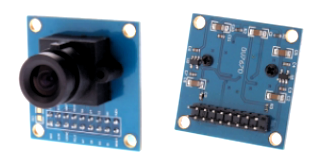
\includegraphics[scale=0.6]{images/camera.png}
    \caption{OV7070 camera module.}\\[1 in]
    \label{fig:my_label}
\end{figure}

\begin{table}[]
    \centering
    \begin{tabular}{|c|c|c|}
        \hline Signal & Usage & Active  \\\hline \hline
         3V3 & 3.3 power & \\\hline
         GND & Ground & \\\hline
         SIOC & Serial command bus clock (upto 400Khz) & Active high, configurable \\\hline
         SIOD & Serial command bus Data & Active high, configurable \\\hline
         VSYNC & Vertical Sync & \\\hline
         HREF & CE output for pixel sampling & \\\hline
         PCLK & Pixel Clock & \\\hline
         XCLK & System clock (10-48 Mhz, Typ. 24 Mhz) & \\\hline
         D0-D7 & Pixel Data & \\\hline
         RESET & Device Reset & Active Low\\\hline
         PWDN & Device Power Down & Active High\\\hline

    \end{tabular}
    \caption{I/O signals of the camera module}
    \label{tab:my_label}
\end{table}
A video is a succession of frames. A frame of the video is a still image taken at an instant of time. A frame is compromised of rows (or lines), and a row is compromised of a number of pixels - whose number on the row equals the number of columns. A pixel is the smallest part of a digital image, and it looks like a colored dot. For example, a simple 4x3 image is shown below.
\begin{figure}[H]
    \centering
    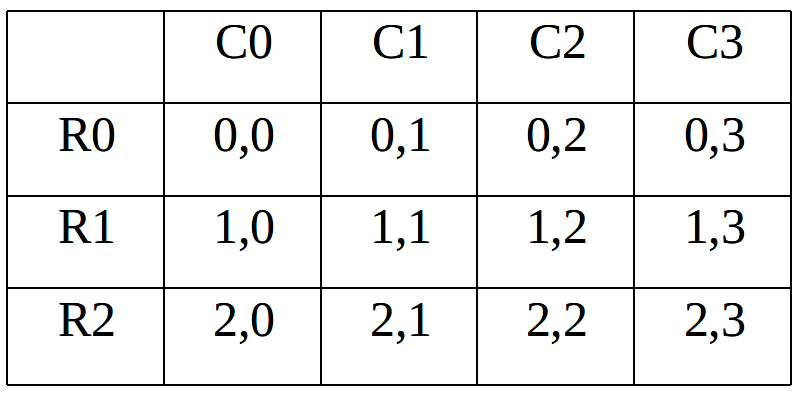
\includegraphics[scale=0.25]{images/column.png}
    \caption{Image with 4x3 pixels}
    \label{fig:my_label}
\end{figure}
There are many pixel formats. Some of the simplest pixel formats include monochrome and RGB. In monochromes images, each pixel is stored as 8 bits, representing gray scale levels from 0 to 255, where 0 is black, 255 is white and the intermediate values are shades of gray. In the RGB color model, any color can be decomposed in Red, Green and Blue light at different intensities. Because a color can be made by mixing Red, Green and Blue, it is called the RGB color system or model. It is also called an "Additive" color system, because it starts at black, and then color is added. Using this model, each pixel must be stored as three intensities of these red, green and blue lights. The most common format is RGB888. In this format each pixel is stored using 24 bits - the red, green and blue channels are stored in 8 bits each:
$$\text{RRRRRRRRGGGGGGGGBBBBBBBB}$$
For instance, the color red would be stored, in binary, as 24 bits as:
$$\text{111111110000000000000000}$$
or, as commonly shown in hexadecimal, as: FF0000\\
However, the RGB formats used by the OV7670 are: RGB565, RGB555 and RGB444. The difference, compared to RGB888 format, is the number of bits assigned to each channel. For example, in the RGB565 format, the red channel is stored as 5 bits, the green channel as 6 bits and the blue channel as 5 bits. These formats take less memory when stored but in exchange sacrifice the number of colors available.\\
Retrieving data from the camera module is relatively simple. As can be seen in the datasheet, and shown in Fig.2.3 and 2.4, signals VSYNC and HSYNC give us the "points of reference" we need to know when pixel data of a frame are being transmitted from the camera module.
\begin{figure}[H]
    \centering
    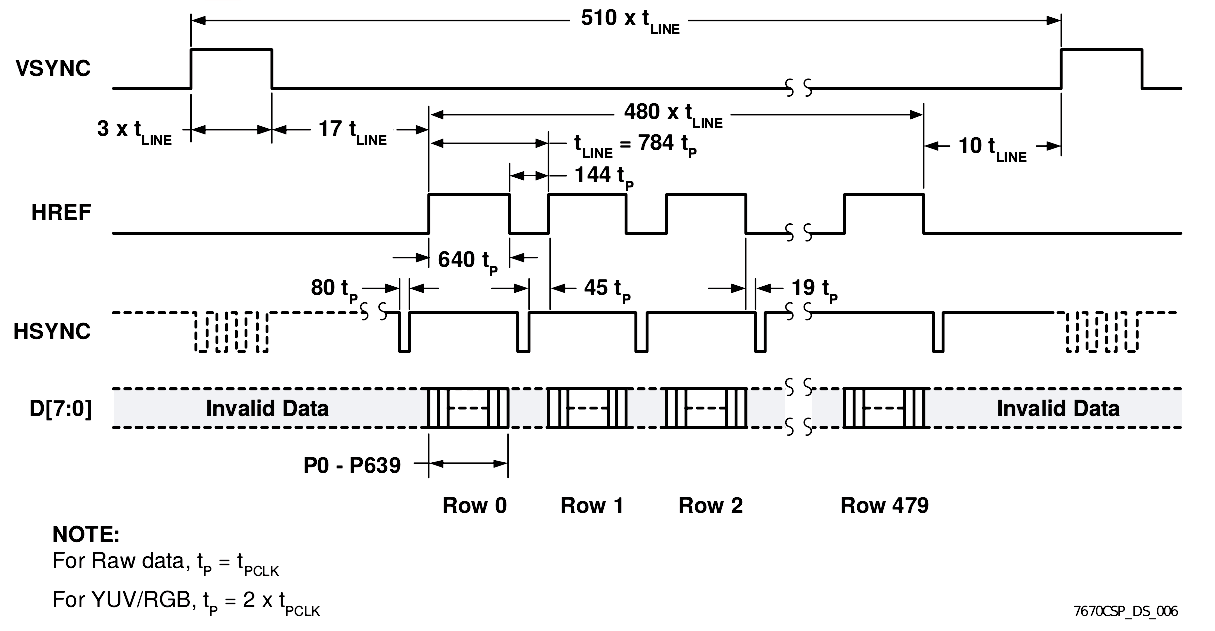
\includegraphics[scale=0.4]{images/Signal.png}
    \caption{VGA frame timing}
    \label{fig:my_label}
\end{figure}
\begin{figure}[H]
    \centering
    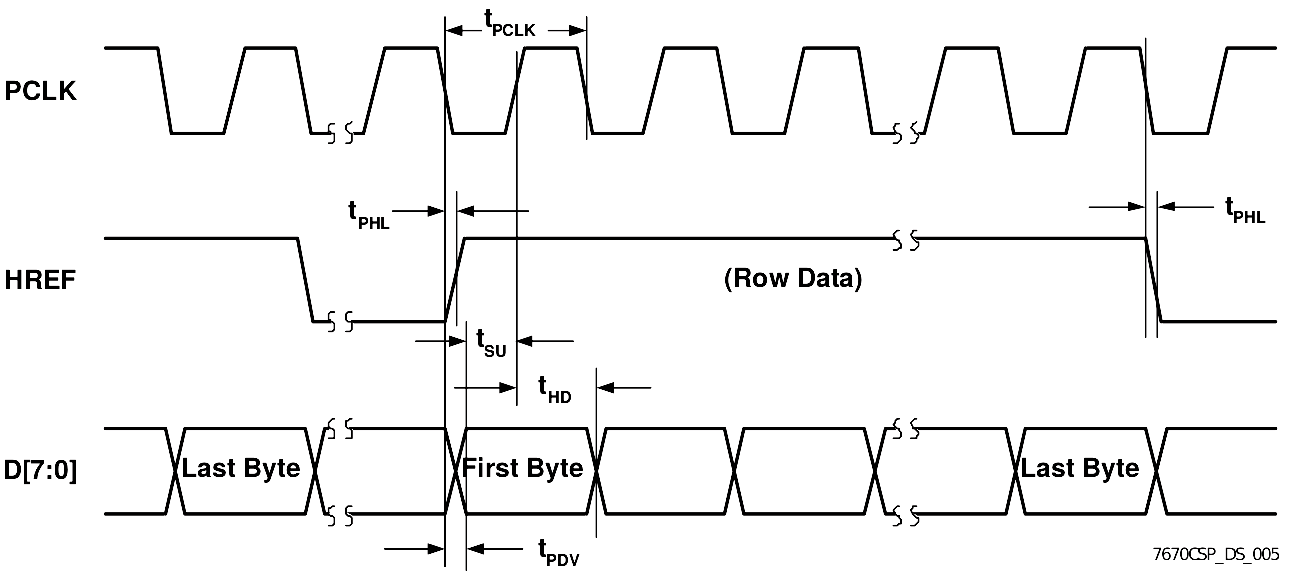
\includegraphics[scale=0.3]{images/timmimg.png}
    \caption{RGB 565 output timing diagram}
    \label{fig:my_label}
\end{figure}
\subsection{Architecture}
We simply build a preliminary design where we simply connect the OV7670 camera module to the FPGA, retrieve video frames from the camera module, store temporarily each image frame's data inside the FPGA, and use that data to drive a VGA monitor connected to the board. We'll complicate this design in follow-up implementations. Note that each implementation is a stand alone design by itself.
\begin{figure}[H]
    \centering
    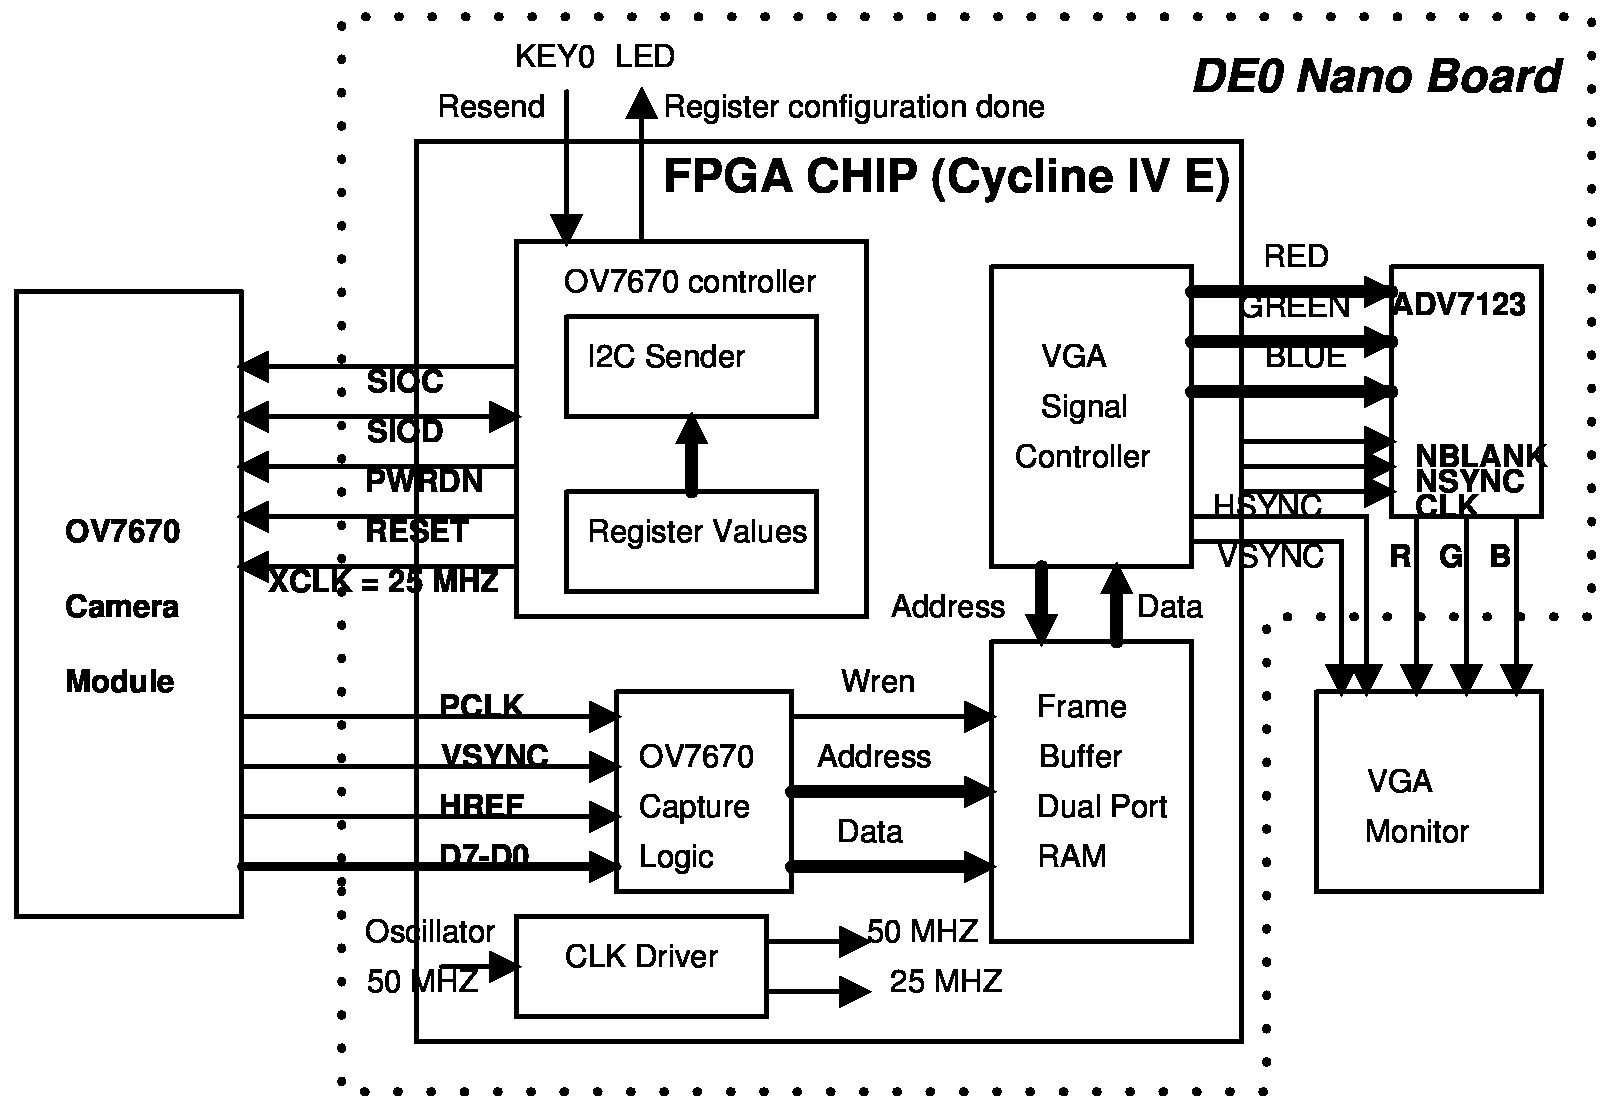
\includegraphics[scale=0.3]{images/vlsi.jpg}
    \caption{Block diagram of the implementation}
    \label{fig:my_label}
\end{figure}
\printbibliography
\end{document}

